\documentclass[a4paper, 14pt]{extarticle}	% general format

%%%% Charset
\usepackage{cmap}							% make PDF files searchable and copyable
\usepackage[utf8x]{inputenc}				% accept different input encodings
\usepackage[T2A]{fontenc}					% russian font
\usepackage[russian]{babel}					% multilingual support (T2A)

%%%% Graphics
\usepackage[dvipsnames]{xcolor}			% driver-independent color extensions
\usepackage{graphicx}						% enhanced support for graphics
\usepackage{wrapfig}						% produces figures which text can flow around

%%%% Math
\usepackage{amsmath}						% American Mathematical Society (AMS) math facilities
\usepackage{amsfonts}						% fonts from the AMS
\usepackage{amssymb}						% additional math symbols

%%%% Typograpy (don't forget about cm-super)
\usepackage{microtype}						% subliminal refinements towards typographical perfection
\linespread{1.3}							% line spacing
\usepackage[left=2.5cm, right=1.5cm, top=2.5cm, bottom=2.5cm]{geometry}
\setlength{\parindent}{0pt}					% we don't want any paragraph indentation
\usepackage{parskip}						% some distance between paragraphs

%%%% Tables
\usepackage{tabularx}						% tables with variable width columns
\usepackage{multirow}						% for tabularx
\usepackage{hhline}							% for tabularx

%%%% Graph
\usepackage{tikz}							% package for creating graphics programmatically
\usetikzlibrary{arrows}						% edges for tikz

%%%% Other
\usepackage{url}							% verbatim with URL-sensitive line breaks
\usepackage{fancyvrb}						% sophisticated verbatim text (with box)
%------------------------------------------------------------------------------

%------------------------------------------------------------------------------
\usepackage{listings}						% typeset source code listings

% Цвета для кода
\definecolor{string}{HTML}{101AF9}			% цвет строк в коде
\definecolor{comment}{HTML}{3F7F5F}		% цвет комментариев в коде
\definecolor{keyword}{HTML}{5F1441}		% цвет ключевых слов в коде
\definecolor{morecomment}{HTML}{8000FF}	% цвет include и других элементов в коде
\definecolor{captiontext}{HTML}{FFFFFF}	% цвет текста заголовка в коде
\definecolor{captionbk}{HTML}{999999}		% цвет фона заголовка в коде
\definecolor{bk}{HTML}{FFFFFF}				% цвет фона в коде
\definecolor{frame}{HTML}{999999}			% цвет рамки в коде

% Настройки отображения кода
\lstset{
	language=Python,						% Язык кода по умолчанию
	morekeywords={*,...},					% если хотите добавить ключевые слова, то добавляйте
	% Цвета
	keywordstyle=\color{keyword}\ttfamily\bfseries,
	stringstyle=\color{string}\ttfamily,
	commentstyle=\color{comment}\ttfamily\itshape,
	morecomment=[l][\color{morecomment}]{\#},
	% Настройки отображения
	breaklines=true,						% Перенос длинных строк
	basicstyle=\ttfamily\footnotesize,		% Шрифт для отображения кода
	backgroundcolor=\color{bk},				% Цвет фона кода
	%frame=lrb,xleftmargin=\fboxsep,xrightmargin=-\fboxsep, % Рамка, подогнанная к заголовку
	frame=tblr								% draw a frame at all sides of the code block
	rulecolor=\color{frame},				% Цвет рамки
	tabsize=2,								% tab space width
	showstringspaces=false,					% don't mark spaces in strings
	% Настройка отображения номеров строк. Если не нужно, то удалите весь блок
	numbers=left,							% Слева отображаются номера строк
	stepnumber=1,							% Каждую строку нумеровать
	numbersep=5pt,							% Отступ от кода
	numberstyle=\small\color{black},		% Стиль написания номеров строк
}

% Для настройки заголовка кода
\usepackage{caption}
\DeclareCaptionFont{white}{\color{сaptiontext}}
\DeclareCaptionFormat{listing}{\parbox{\linewidth}{\colorbox{сaptionbk}{\parbox{\linewidth}{#1#2#3}}\vskip-4pt}}
%\captionsetup[lstlisting]{format=listing,labelfont=white,textfont=white}
\renewcommand{\lstlistingname}{Листинг} % Переименование Listings в нужное именование структуры
%------------------------------------------------------------------------------

\begin{document}

%------------------------------------------------
\begin{titlepage}
\thispagestyle{empty}

\begin{center}
Санкт-Петербургский политехнический университет Петра Великого\\
Институт Информационных Технологий и Управления \\*
Кафедра компьютерных систем и программных технологий \\*
\hrulefill
\end{center}

\vspace{10em}

\begin{center}
\Large Отчёт по самостоятельно работе\\по предмету «Теория распознавания образов» \\
\end{center}

\vspace{1em}

% \linebreak
\begin{center}
\textsc{\textbf{Локализация и отслеживние лиц на изображении}}
\end{center}

\vspace{16em}

\begin{flushleft}
Работу выполнил студент гр. 53501/3 \hrulefill Мартынов С. А. \\
\vspace{1.5em}
Работу принял преподаватель \hrulefill Никитин К. В. \\
\end{flushleft}

\vspace{\fill}

\begin{center}
Санкт-Петербург \\
2015
\end{center}

\end{titlepage}
%------------------------------------------------
\setcounter{page}{2}
\tableofcontents

%------------------------------------------------------------------------------

\newpage
\section*{Введение}
\addcontentsline{toc}{section}{Введение}

Локализация человеческого лица с последующей идентификацией давно находится в списке наиболее важных задач для исследователей в области систем машинного зрения и искусственного интеллекта. Множество исследований, проводимых ведущими научными центрами, так и не позволило создать универсальную систему компьютерного зрения, способную к локализации и распознаванию лица человека при различных условиях.

Причиной тому явилось сразу множество факторов, среди которых:
\begin{itemize}
\item высокая вариативностью лиц, обусловленной анатомическими особенностями людей;
\item различный уровень освещенности объектов, зависящих от типа, количества и характеристик направленности источников света;
\item необходимость обнаружения лиц, имеющих различное пространственное положение.
\end{itemize}

Зачастую особенности системы, использующей локализацию и распознавание лиц может накладывать дополнительные ограничения на скорость работы (близкой к реальному времени), аппаратным ресурсам (процессор, объём памяти) и экономичности (аккумулятора).

Кроме скоростных характеристик, от алгоритма требуется обеспечение малого (порядка 5\%) количества ложных распознаваний. В системах, реализующих существующие методы распознавания, при увеличении уровня распознаваний свыше 90\% наблюдается существенный рост числа ложных решений, что затрудняет их практическое использование. Прежде чем распознавать лицо, необходимо убедиться в его присутствии на изображении. Для чего применяются известные методы обнаружения и распознавания лиц на изображениях (метод главных компонент, нейронные сети, метод опорных векторов). Результативность применения метода определяется спецификой решаемой задачи. Поэтому построение метода распознавания лиц, обеспечивающего высокий уровень достоверности решения при отсутствии ограничений на исходные изображения, является весьма актуальной задачей.

Целью данной работы является обзор основных методов обнаружения лиц (под обнаружением лиц на изображении будем понимать процесс локализации областей изображения, содержащих лица людей; границы искомых областей в в общем случае размыты, однако чаще всего подразумевается минимальный описывающий прямоугольник), обеспечивающих повышение достоверности распознавания объектов анализа, снижение уровня ложных распознаваний, уменьшение времени обучения классификатора и времени предварительной обработки изображения.

%------------------------------------------------------------------------------

\newpage
\section{Признаки изображений}

Вычисление признаков изображения является одним из важнейших аспектов при распознавании визуальных образов. Признак в данном контексте это произвольные дескрипторы изображения, полученные в результате обработки исходных данных. Качество детектирования определяется информативностью выделенных признаков, а вычислительная сложность алгоритмов выделения -- скоростью работы системы распознавания. В самом простом случае, признаком может являться яркость или цвета пикселей, составляющих исследуемое изображение.

Имеется множество различных примеров классификации признаков по типу, но обычно выделяют три основные категории:
\begin{itemize}
\item яркостные -- базируются на перепадах яркости в пикселях;
\item текстурные -- описываются с помощью повторяющихся базовых элементов текстур;
\item геометрические -- описывают фрагменты фигур и контуров, присутствующих на изображении.
\end{itemize}

Тип вычисляемых признаков определяется содержимым изображения, которое надо описать. Обобщенное человеческое лицо, как графический паттерн, из-за своей сложности может быть описано сразу всеми типами признаков. 

\subsection{Признаки Хаара}

Вейвлеты Хаара -- это семейство базисных функций, открытое в начале XX века Альфредом Хааром. Вейвлеты Хаара ортогональны, обладают компактным носителем, хорошо локализованы в пространстве, являются кусочно-постоянными функциями с разрывами 1-го рода. Из-за своей простой и быстрой формулы расчета они повсеместно применяются в задачах анализа нестационарных сигналов.


Рассмотрим множество кусочно-постоянных функций, определенных на интервале $[0, 1)$, состоящем из $2^l$ подинтервалов равной длины. Пусть функции, определенные на всем единичном интервале, образуют пространство $V^0$; кусочно постоянные функции, одна часть каждой из которых определена на интервале $[0, \frac{1}{2})$, а другая на $[\frac{1}{2}, 1)$ образуют пространство $V^1$ и т.д. Таким образом, пространство $V^l$ содержит все кусочно-постоянные функции, определенные на всех $2^l$ подинтервалах единичного интервала. Базис Хаара представляет собой множество функций, определенных для каждого пространства $V^l$ . Базисные функции называются масштабирующими функциями и порождаются сдвигами и растяжениями прямоугольного импульса.

\begin{gather}
\varphi(x) =
  \begin{cases}
    1,\qquad 0\le x \le 1,\\
    0,\qquad otherwise.
 \end{cases}
\end{gather}

\begin{gather}
\varphi_{l,t}(x) = 2^{1/2}\varphi(2^lx-t)
\end{gather} 

Масштаб определяется множителем $2^{l/2}$, а сдвиг задается параметром $t = 0 \ldots{} 2^{l-1} - 1$. Интеграл от масштабирующей функции на интервале $[-\infty, +\infty]$ равен единице. Соответствующий набор вейвлет-функций Хаара, ортогональный масштабирующим функциям, определяется посредством смещения и растяжения своего материнского вейвлета.

\begin{gather}
\psi(x) =
  \begin{cases}
    1,\qquad 0\le x \le \dfrac{1}{2},\\
    -1,\qquad \dfrac{1}{2}\le x \le 1,\\
    0,\qquad otherwise.
 \end{cases}
\end{gather}

\begin{gather}
\psi_{l,t}(x) = 2^{1/2}\psi(2^lx-t)
\end{gather} 

Интеграл от вейвлет-функции на интервале $[-\infty, +\infty]$ принимает нулевое значение.

Одномерный базис Хаара, заданный в $V^2$, может быть распространен на плоскость двумя способами. Стандартная композиция получается, когда одномерное вейвлет-преобразование применяется для каждого измерения поочередно: новым базисом служат всевозможные тензорные произведения функций $\psi_{l,t}(\bullet)$. Нестандартный базис выводится путем смещений и растяжений двумерной масштабирующей функции (5) и трех двумерных материнских вейвлетов.

\begin{gather}
\varphi(x,y)=\varphi(x)\varphi(y)
\end{gather}

\begin{gather}
\psi^m(x,y) =
  \begin{cases}
    \psi(x)\varphi(y),\qquad m=1,\\
    \varphi(x)\psi(y),\qquad m=2,\\
    \psi(x)\psi(y),\qquad m=3.
 \end{cases}
\end{gather}

Такой подход имеет преимущества перед стандартной композицией, поскольку обеспечивает лучшее пространственное разрешение за счет некоторой избыточности базиса (рис. 1). При одномерном преобразовании расстояние между соседними вейвлетами $\psi_{l,t}(x)$ составляет $2^l$, в стандартном двумерном базисе -- $2^{l-1}$, а в нестандартном -- $2^{l-2}$.

\begin{figure}[h!]
\centering
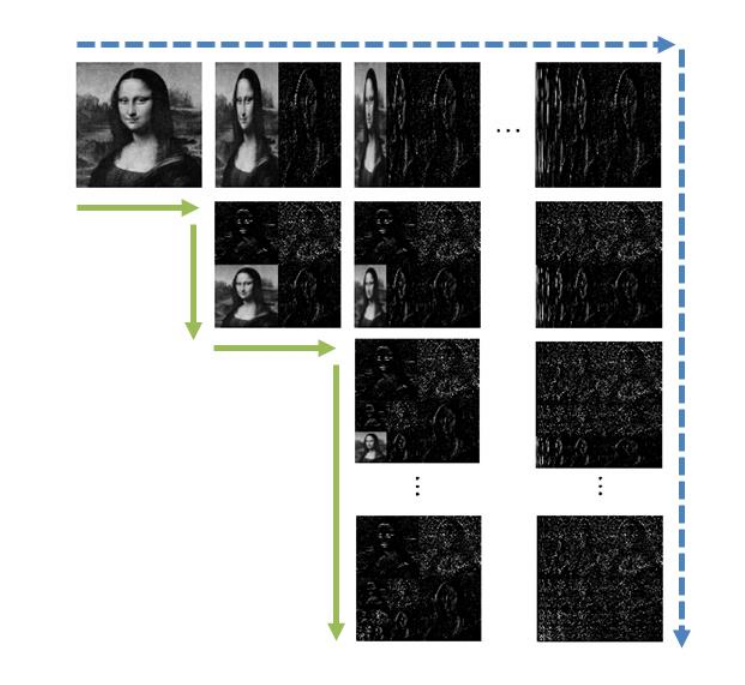
\includegraphics[scale=0.6]{res/pic001}
\caption{Пример вейвлет-декомпозиции двумя способами: стандартным (пунктирная стрелка) и нестандартным (сплошная стрелка)}
\end{figure}

На рис. 2 схематично представлены материнские вейвлеты, полученные по формуле (6). Темная область соответствует отрицательным значениям вейвлета, светлая -- положительным.

\begin{figure}[h!]
\centering
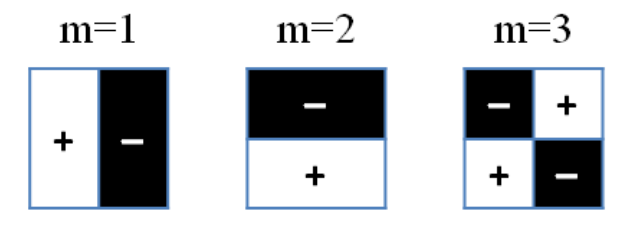
\includegraphics[scale=0.6]{res/pic002}
\caption{Три двумерных материнских вейвлета}
\end{figure}

Признаки Хаара -- признаки цифрового изображения, вычисляемые с помощью функций, схожих по своей структуре с двумерными вейвлетами Хаара. Специалистами было предложено использовать материнские вейвлеты Хаара в качестве ядер для свертки исходного изображения. Каждый вычисляемый признак $H$ представлен комбинацией прямоугольников $h_i$. При подсчете признака окно $h$ скользит по изображению, и вычисляется среднее значение пикселей, покрываемых каждым прямоугольником -- $\mu(i)$ . Прямоугольникам соответствуют веса $w_i \in \{−1, +1\}$, определяющие с каким знаком войдет среднее значение пикселей в общую сумму. Согласно свойству интеграла от масштабирующих функций, веса удовлетворяют условию нулевой суммы:

\begin{gather}
\sum\limits_{k=1}^N w_i=0
\end{gather}

Выражение для вычисления признака имеет следующий вид:

\begin{gather}
H = \sum\limits_{k=1}^N w_i \mu_i
\end{gather}

На рисунке 3 изображены примеры расширенных признаков Хаара, предложенных Виолой и Джонсом (верхний ряд) и Ленхард (нижний ряд).

\begin{figure}[h!]
\centering
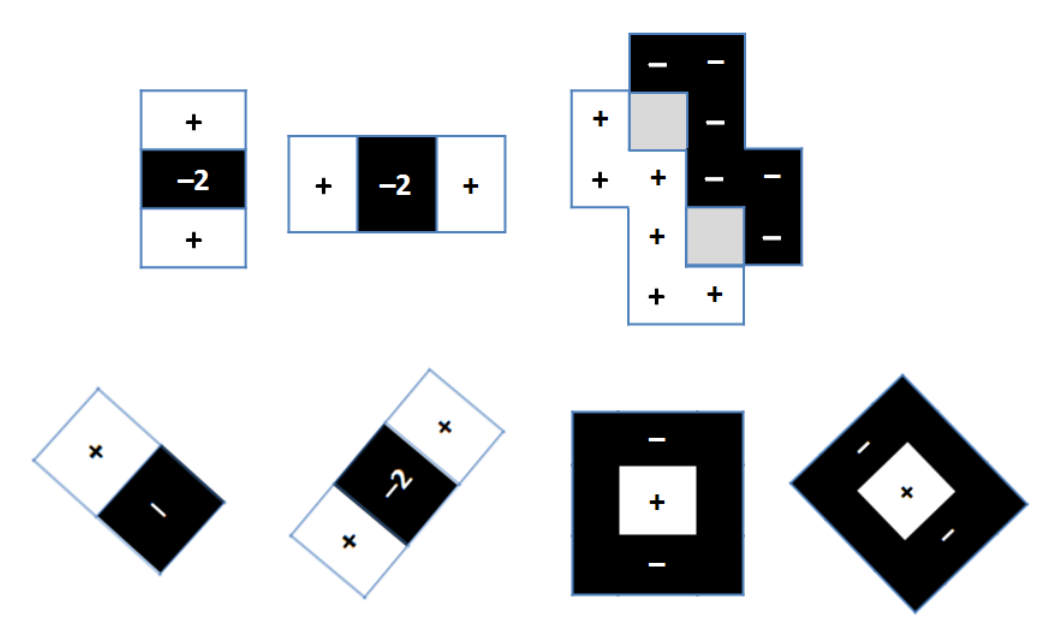
\includegraphics[scale=0.45]{res/pic003}
\caption{Расширенный набор признаков Хаара}
\end{figure}

В пользу признаков Хаара говорит наличие для них эффективных вычислительных схем. Виола и Джонс предлагают использовать интегральное изображение для ускорения процедуры подсчета признаков. Интегральное изображение $\overline{\overline{I}}$ это матрица той же размерности, что и исходное изображение $I$, элементы которой определяются следующим образом:

\begin{gather}
\overline{I}(x,y) = \sum\limits_{\substack{x' \le x\\y' \le y}} I(x',y')
\end{gather}

Тогда среднее значение $\mu_i$ для прямоугольника $h_i$ с вершинами в точках $A_i$ , $B_i$ , $C_i$ , $D_i$ с площадью $S_i$ (рис 1) может быть посчитано за четыре арифметические операций над пикселями интегрального изображения:

\begin{gather}
\mu_i = (\overline{I}(A_i) + \overline{I}(B_i) - \overline{I}(C_i) - \overline{I}(D_i)) / S_i
\end{gather}

Для признаков Ленхард, повернутых на $45\,^{\circ}$, также существует быстрая схема вычислений. Для этого используется понятие таблицы суммированных областей, аналогичное определению интегрального изображения, выраженного формулой (9). Для вычисления таких признаков Ленхард вводится понятие таблицы суммированных областей, которые повернуты на угол, вычисляемой по следующей формуле:

\begin{gather}
\overline{\overline{I}}(x,y) = \sum\limits_{\substack{x' \le x\\x' \le x - |y' - y|}} I(x',y')
\end{gather}

Среднее значение $\mu_i$ для прямоугольника $h_i$ с вершинами в точках $A_i$ , $B_i$ , $C_i$ , $D_i$ с площадью $S_i$ и углом поворота $\alpha_i = 45\,^{\circ}$ может быть также вычислено по формуле (10) для $\overline{I} = \overline{\overline{I}}$.

\subsection{Локальные бинарные шаблоны}

Порядковое измерение контраста (ordinal contrast measure) является порождением простого концепта: относительное важнее абсолютного. При анализе различных изображений мы можем отмечать значительные изменения абсолютных величин: цветов, яркости, текстурных элементов. Однако, взаимные порядковые отношения между соседними величинами, отражающие структуру изображенных объектов, подвержены меньшим изменениям. Порядковое кодирование контраста (ordinal contrast encoding) используется для вычисления существенных контрастных различий (contrast polarity) между двумя пикселями или регионами изображений. Оператор ставит в соответствие паре пикселей 1, если первый пиксель ярче второго или 0, в противном случае. Такой код удобен для вычислений, а информационная энтропия измерений максимальна, поскольку для случайных паттернов практически равновероятны значения 0 и 1.

Операция   порядкового   кодирования   контраста $T \equiv T(X)$ обладает  следующими свойствами инвариантности:

\begin{gather}
T(X) \equiv T(X+a) \equiv T(X \times a) \equiv T(X^a), \\
a \equiv const > 0 \nonumber
\end{gather}

Census-преобразование (рис. 4) проецирует локальное окружение заданного  пикселя  в  битовую  строку.  Полученная  битовая  строка  может быть использована  в  качестве  дескриптора  области  изображения. Обозначим  через $(x_c, y_c)$ координаты  центрального  пикселя, $(x_p, y_p)$ -- координаты  смежного пикселя, $f(\bullet)$ -- значение яркости пикселя в точке с заданными координатами. Тогда census-преобразование может быть представлено следующим образом:

\begin{gather}
T(X) = \otimes_{p=0}^{p-1}s(f(x_p, y_p)-f(x_c, y_c))
\end{gather}

\begin{gather}
s(x) =
  \begin{cases}
    1,\qquad x < 0,\\
    0,\qquad x \ge 0.
 \end{cases}
\end{gather}

\begin{figure}[h!]
\centering
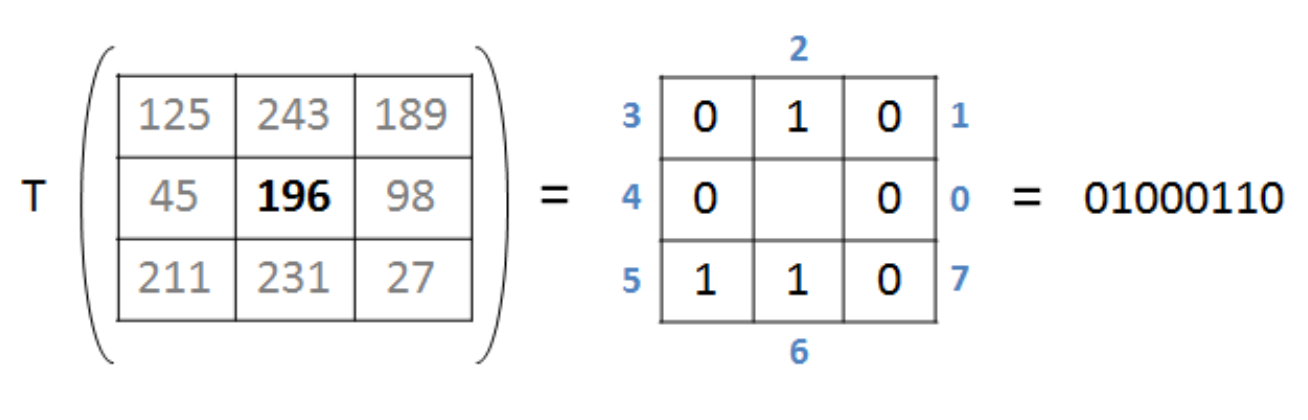
\includegraphics[scale=0.35]{res/pic004}
\caption{Census-преобразование}
\end{figure}

В качестве метрики схожести между census-образами пикселей изображений, используется расстояние Хэмминга, то есть рассчитывается число различающихся битов  в  соответствующих  битовых строках.  Основное  ограничение census-преобразования  в  том,  что  оно  охватывает малый  регион  анализируемого изображения вблизи центрального пикселя -- этого может оказаться недостаточно для выделения ключевых текстурных характеристик.

Обобщенный случай census-преобразования -- метод локальных бинарных шаблонов (ЛБШ), который был предложен Пиетикайненым. Количество соседних  точек,  участвующих  в  построении  дескриптора,  и  их  удаленность  от центрального пикселя определяются параметрами P и R соответственно:

\begin{gather}
LBP_{P,R}(x_c, y_c) =  \sum\limits_{p=0}^{P-1}s(f(x_p, y_p)-f(x_c, y_c))2^P
\end{gather}

Каждому  анализируемому  множеству  пикселей  оператор ЛБШ ставит  в соответствие   натуральное   число,   определяющееся   из   равенства (15). Принципиальным отличием ЛБШ от Census-преобразования является то, что ЛБШ-преобразование может применяться к соседним пикселям, лежащим на некоторой окружности  радиуса $R \ge 1$ c центром  в  пикселе $x_c$ (рисунок 5).  Координаты пикселей $x_p$ могут быть рассчитаны исходя из соотношений:

\begin{gather}
s(x) =
  \begin{cases}
    x_p=x_c + R \cos \frac{2 \pi p}{P} \\
    y_p=y_c - R \sin \frac{2 \pi p}{P}
 \end{cases}
\end{gather}

\begin{figure}[h!]
\centering
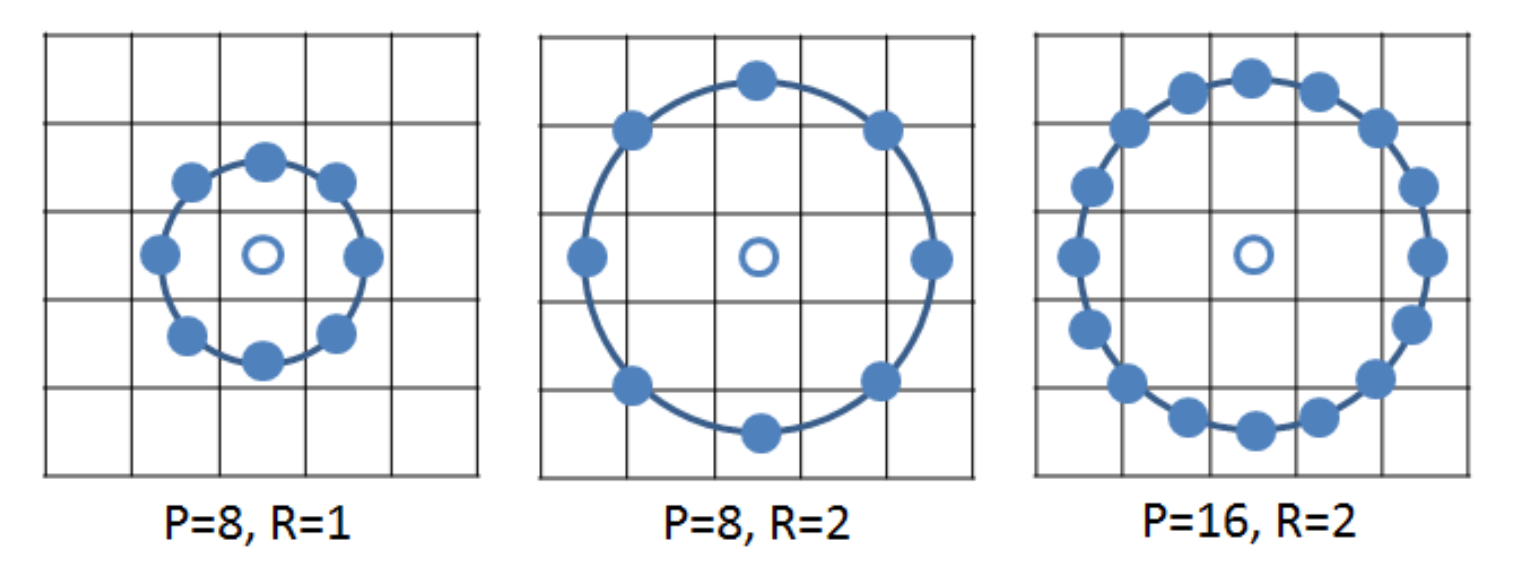
\includegraphics[scale=0.33]{res/pic005}
\caption{LBP-преобразование с различным радиусом и количеством соседе}
\end{figure}

Если  координаты  точки $(x_p, y_p)$ не  соответствуют  центру  какого-либо пикселя изображения, то значение яркости в данной точке может быть получено с помощью интерполяции. Одним из самых простых и распространенных способов является  билинейная  интерполяция.  Если  положить,  что  четыре  ближайших  к $(x_p, y_p)$ пикселя лежат на вершинах единичного квадрата, $x = x_p - | x_p |$, $y = y_p - | y_p |$ , то значение яркости в точке $(x_p, y_p)$ может быть вычислено по значениям пикселей в вершинах квадрата:

\begin{gather}
f(x_p, y_p) \approx 
\begin{bmatrix}
  1-x & x
\end{bmatrix}
\begin{bmatrix}
  f(0,0) & f(0,1)\\
  f(1,0) & f(1,1)
\end{bmatrix}
\begin{bmatrix}
  1-y\\
  y
\end{bmatrix}
\end{gather}

При P=8, R=1 формула ЛБШ принимает классическую форму. Многомасштабный анализ, основанный на ЛБШ, может производиться  двумя способами. В первом случае меняется радиус R оператора ЛБШ-преобразования. Во  втором  случае  уменьшается  размерность  исходного  изображения  с последующим применением ЛБШ-оператора фиксированного радиуса. 
Оператор (15),  строго  говоря,  не  является  инвариантным  к  поворотам исходного изображения. Предлагается проецировать область пикселя в  битовую  строку,  записанную  как  циклический  код.  Случайно  совершая циклические  перестановки,  ищется  совпадение  с  одним  из  наперед  заданных бинарных шаблонов. Оператор $LBD_{P,R}^{ri}$ возвращает номер совпавшего с битовой строкой  бинарного  шаблона.  Для  случая,  когда $P=8$ имеется ряд унифицированных  шаблонов  (uniform patterns), которые 
получаются из циклических сдвигов нескольких категорий битовых строк (рисунок 6): 
\begin{enumerate}
\item Линии (lines): 01111111, 00000001.
\item Углы (corners): 00111111, 00011111, 00001111, 00000011.
\item Край (edge): 00000111.
\end{enumerate}

\begin{figure}[h!]
\centering
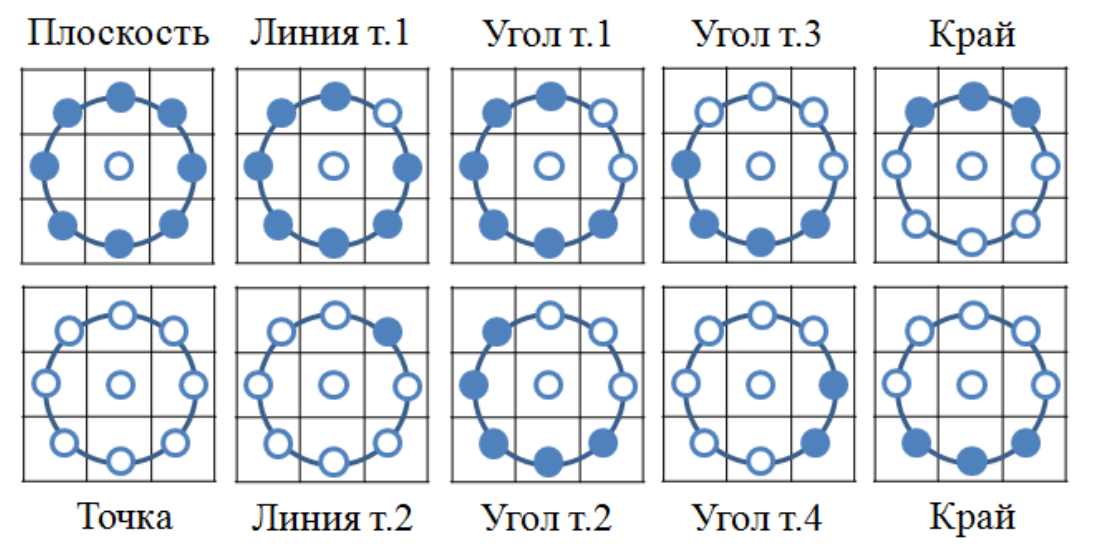
\includegraphics[scale=0.45]{res/pic006}
\caption{Примеры унифицированных шаблонов}
\end{figure}

Перечисленные категории образуют 56 паттернов, к ним добавляется еще два шаблона,  которые  не  варьируются  циклическим  смещением:  11111111 --
плоскость  (flat),  00000000 -- точка  (spot).  Оператор,  использующий  58 унифицированных шаблонов для описания области изображения, обозначается как $LBD_{P,R}^{ri2u}$.

В качестве дескриптора для анализа изображений используется гистограмма ЛБШ-образов пикселей. Пусть область значений $A$ оператора $LBD_{P,R}^{ri2u}$ разбита на равные промежутки: 
$ A = \cup_i(a_{i-1},a_i]$

\begin{gather}
n_{P,R}(i)=\sum\limits_{j=1}^{N}1_{\{LBD_{P,R}^{ri2u}(x_{c_j},y_{c_j})\in(a_{i-1},a_i]\}}
\end{gather}

$n_{P,R}(i)$ -- число значений, попавших в i-ый интервал. Пусть $N = |A|$. Тогда нормализованная гистограмма ЛБШ-признаков принимает следующий вид:

\begin{gather}
h_{P,R}(i)=\frac{n_{P,R}(i)}{N \times (a_i - a_{i-1})}
\end{gather}

\subsection{Двухмерное косинусное преобразование}

При выборе признаков необходимо учитывать следующие характеристики: устойчивость к условиям освещения, чувствительность к цифровому сжатию, вычислительная сложность. Помимо прочего, важным фактором является размер выборки признаков, т.е. количество однотипных признаков, выделяемых на одном статическом изображении. Косинусное преобразование – подходящий метод для выделения признаков изображения с точки зрения вышеперечисленных факторов, поскольку обладает высокой устойчивостью к условиям освещения высокочастотным шумам, является вычислительно простым алгоритмом.

\begin{gather}
f(u, v) = \frac{2}{N} C(u)C(v)\Big(\sum\limits_{x=0}^{N-1}\sum\limits_{y=0}^{N-1}f(x, y) \cos \frac{(2x+1)u\pi}{2N} \cos \frac{(2y+1)v\pi}{2N} \Big)
\end{gather}

\begin{gather}
C(z) =
  \begin{cases}
    \frac{1}{\sqrt{2}}, \quad z = 0 \\
    1, \quad z \neq 0
 \end{cases}
\end{gather}
где $f(x, y)$ -- квадратная область $N \times N$ исходного изображения, подвергающегося
косинусному преобразованию, $u, v$ -- координаты вычисляемого признака.

Применение двухмерного дискретного косинусного преобразования (ДКП-2) ко всей области изображения не позволяет извлекать информацию о частотных характеристиках отдельных областей изображения (рисунок 7). Кроме того, для некоторых вероятностных алгоритмов требуется большое число признаков, отражающих локальную информацию, для эффективного обучения. Рассмотрим применение ДКП-2 блочно, с окном фиксированного размера и постоянной величиной сдвига $S$ (рисунок 8), как в алгоритме JPEG.

\begin{figure}[h!]
\centering
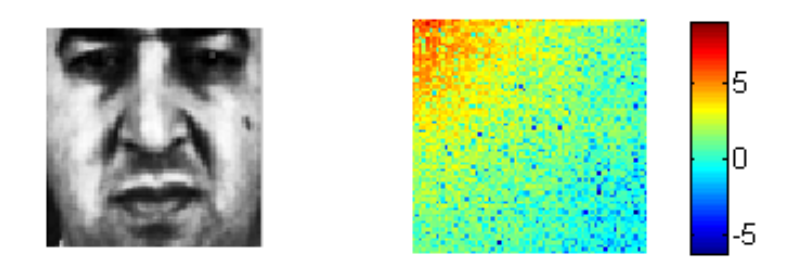
\includegraphics[scale=0.55]{res/pic007}
\caption{Пример вычисления ДКП-2: оригинальное изображение (слева), абсолютные значения коэффициентов ДКП-2 (справа)}
\end{figure}

Так, для изображения размером $96 \times 96$ пикселей оконное ДКП-2 при $N=8$ и $S=4$ производит 484 64-мерных вектора коэффициентов.

\begin{figure}[h!]
\centering
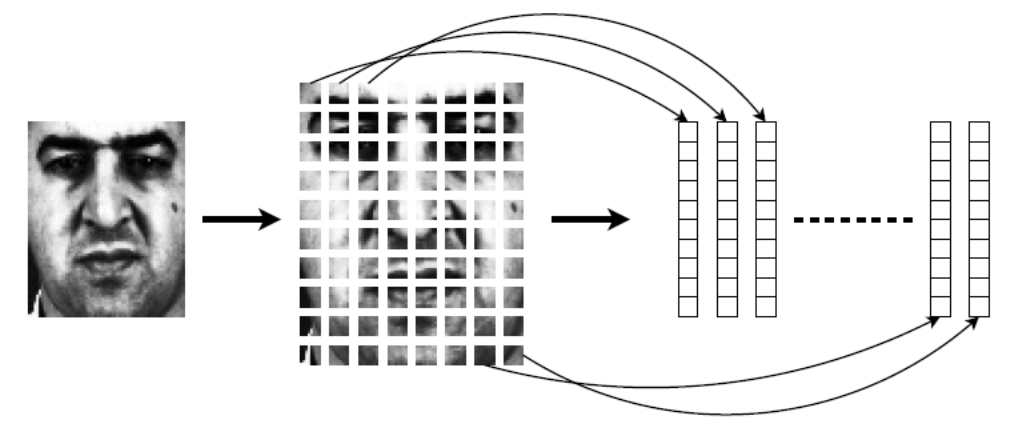
\includegraphics[scale=0.48]{res/pic008}
\caption{Формирование матрицы признаков посредством оконного ДКП-2}
\end{figure}

Исследуя зависимость качества работы системы распознавания, построенной на признаках ДКП-2, от размера окна преобразования N и базы лиц, оказывается, что оптимальный размер окна преобразования сильно изменяется при тестировании на различных базах, от $8 \times 8$ (база MOBIO) до $20 \times 20$ (база SCface), и зависит от условий, в которых была собрана конкретная база, в том числе и от размера изображений лиц.

Большая часть полезной информации сосредоточена в низкочастотных коэффициентах изображения, в то время как шумовые составляющие обычно выражаются высокочастотными. Поэтому в ряде случаев, связанных со сжатием изображения или извлечением информативных данных, размерность вектора признаков F экспериментально ограничивают сверху.

На этапе формирования векторов признаков оконного ДКП-2 (рисунок 8) каждая матрица признаков, получаемая путем применения ДКП-2 к локальной области, разворачивается в многомерный вектор коэффициентов. Существует множество способов формирования такого вектора, наиболее распространенным является способ "zig-zag" (рисунок 9).

\begin{figure}[h!]
\centering
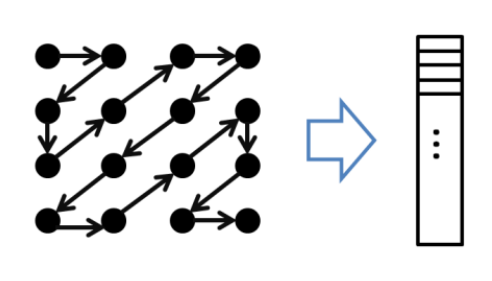
\includegraphics[scale=0.45]{res/pic009}
\caption{Способ "zig-zag" развертки матрицы признаков в вектор}
\end{figure}

\newpage
Особенность данного подхода заключается в том, что не отдается предпочтение какому-либо из двух направлений, в которых разворачивается набор коэффициентов ДКП-2.

%------------------------------------------------------------------------------

\newpage
\section{Методы бинарной классификации признаков}

Детектирование лиц на изображении относится к задачам бинарной классификации. Пусть $X = \{x_i\}$ -- множество произвольных областей изображения, $Y = \{−1, 1\}$ -- множество меток классов, $k \in K$ -- алгоритмы бинарной классификации, тогда процесс классификации областей может быть записан следующим образом:

\begin{gather}
X\xrightarrow{k}Y
\end{gather}

Предположим, что для некоторых $\hat{x}_j \in \hat{X} \subset X$ известны ответы $\hat{y}_j \in \hat{Y} \subset Y$, $j = 1, \dots, L$. Отображение вида

\begin{gather}
(\hat{X} \times \hat{Y})^L \rightarrow k
\end{gather}
называется алгоритмом обучения классификатора k.

Для оценки производительности классификатора вводится функция потерь $L(k, x)$ -- величина ошибки алгоритма k на элементе x из множества X. При решении задач бинарной классификации часто используется функция потерь от одного аргумента:

\begin{gather}
L(k, x) = L(y \ast k(x))
\end{gather}

где y -- метка класса элемента x.

\subsection{Композиции классификаторов}

Рассмотрим изображение $X$ и функцию $f_i(x)$, где $x$ -- некоторая произвольная область изображения, а $f_i$ -- скалярная функция вычисления признака от заданной области. Согласно представленным в предыдущих разделах описаниям видов признаков, $f_i$ может вычисляться как свертка изображения с одним из вейвлетов
Хаара по формуле (10)(22) или являться i-ым бином гистограммы признаков ЛБШ (19). Применительно к ДКП-2 $f_i$ можно представить как i-ый коэффициент преобразования $F(u, v)$ при фиксированном положении окна.

Набор всевозможных функций вида (25) будем называть множеством слабых (элементарных) классификаторов

\begin{gather}
k_i(x, a_i) = k_i(f_i, x, p_i, \theta_i) = 
  \begin{cases}
    1, \quad p_if_i(x) < p_i \theta_i \\
    -1, \quad \text{иначе}
 \end{cases}
\end{gather}
где $\theta$ -- порог принятия решения, $p \in \{−1, 1\}$ определяет направление знака неравенства, $k_i \in K$, $a_i = \{f_i, p_i, \theta_i\}$ -- набор указанных параметров. Применительно к задаче детектирования лиц на изображениях, множество $K$ можно представить как совокупность независимых детекторов, анализирующих каждую область изображения. Поскольку заранее неизвестно, какие из признаков окажутся наиболее информативными для описания конкретного паттерна лица, то на этапе обучения алгоритма детектирования целесообразно проверить все доступные элементарные детекторы и попытаться сформировать один "сильный" детектор.

Процедура последовательного построения композиции элементарных классификаторов, когда каждый последующий классификатор стремится компенсировать недостатки композиции всех предыдущих, получила название бустинга (boosting). Алгоритм бустинга является жадным алгоритмом -- на каждом шаге, компенсируя ошибку предыдущей композиции, он принимает локально оптимальное решение, будучи уверенным, что итоговое решение будет также
оптимальным. Цель бустинга -- построение композиции $s_D$ слабых алгоритмов $k_i$:

\begin{gather}
s_D(x)=s(k_1(x),k_2(x),\dots,k_L(x))
\end{gather}

Процесс последовательного обучения композиции может иметь следующие критерии останова:
\begin{itemize}
\item построено заданное количество элементарных классификаторов L,
\item достигнута заданная точность на обучающей выборке,
\item достигнутую точность не удается улучшить на протяжении T шагов.
\end{itemize}

Закономерным результатом развития данного подхода стал алгоритм адаптивного бустинга. Количество классификаторов в композиции стало произвольным, а каждый последующий классификатор строится на ошибочных ответах предыдущих (адаптивность), используя одну и ту же базу для обучения. Для алгоритма адаптивного бустинга впервые была доказана теорема бустинга, которая задавала оптимальный способ формирования композиции слабых классификаторов в виде взвешенной суммы.

\subsection{Адаптивный бустинг и метод Виолы-Джонса}

Рассмотрим три модификации алгоритма адаптивного бустинга, применяющихся для построения детектора лиц:
\begin{itemize}
\item Дискретный адаптивный бустинг (Discrete Adaptive Boosting, DAB).
\item Вещественный адаптивный бустинг (Real Adaptive Boosting, RAB).
\item Плавный адаптивный бустинг (Gentle Adaptive Boosting, GAB).
\end{itemize}

Алгоритм DAB был предложен Фройндом и Шапире. При построении композиции классификаторов алгоритмом DAB используются два типа весов: коэффициенты взвешенного голосования классификаторов $c_m \in C$ и веса обучающих сэмплов $w_i \in W$. На каждой итерации алгоритм DAB увеличивает веса тех наблюдений $x_i$, на которых классификаторы чаще ошибаются. Доля решения классификатора в общем голосовании $c_m$ определяется точностью его решений на выборке $X$. Формула взвешенного голосования DAB выглядит следующим образом:

\begin{gather}
s_D(x)=\sum\limits_{m=1}^{M}c_mk_m(x)
\end{gather}

Перед началом итеративного процесса веса объектов полагаются одинаковыми (28). На каждой итерации выполняется перенормировка весов с целью выполнения условия (29).

\begin{gather}
w_i=\frac{1}{N},\quad i = 1, \dots, N
\end{gather}

\begin{gather}
\sum\limits_{i=1}^{N}w_i=1
\end{gather}

Для каждого классификатора из множества K выполняется три шага:
\begin{enumerate}
{\item Сначала на выборке X обучается классификатор $k_m(x, a_m)$ (в более общем случае $k_m = k_m (x, a_m , W))$:

\begin{gather}
k_m=\underset{a_m} {\mathrm{argmax}}\sum\limits_{i=1}^{N}L(y_i w_i k(x_i, a_m))
\end{gather}

}
{\item Затем, рассчитывается ошибка m-го классификатора на всем обучающем множестве.

\begin{gather}
\mathcal{E}_m= \frac{1}{N} \sum\limits_{i=1}^{N} 1_{\{ y_i \neq k_m(x_i) \}}
\end{gather}

Согласно основной теореме бустинга, определяется вес классификатора $k_m$ в финальной композиции:

\begin{gather}
c_m = \frac{1}{2} \ln \dfrac{1-\mathcal{E}_m}{\mathcal{E}_m}
\end{gather}

}
{\item Наконец, обновляются веса для каждого сэмпла из базы обучения. При изменении весов используется экспоненциальная функция потерь: $L(k, x) = e^{-y \ast k(x)}$.

\begin{gather}
w_i = w_i e ^{c_m 1_{\{y_i \neq k_m(x_i)\}}}
\end{gather}

\begin{gather}
w_i = \dfrac{w_i}{\sum_{j=1}^{N}w_j}
\end{gather}

}
\end{enumerate}

RAB является вероятностным обобщением алгоритма DAB. Дискретное множество ответов $Y = \{−1, 1\}$ заменяется на непрерывную оценку $f_m(x)$, знак которой определяет класс распознанного объекта, а модуль -- степень "уверенности" классификатора. Голосование классификаторов задается суммой вкладов $f_m$:

\begin{gather}
s_R(x) = \sum\limits_{m=1}^{M} f_m(x)
\end{gather}

На втором шаге m-ой итерации, после обучения классификатора на выборке X, рассчитывается оценка вероятности положительного класса:

\begin{gather}
p_m(X) = \hat{P}_w(y = 1|x)
\end{gather}

Вклад m-го классификатора в общее решение определяется логит-функцией от вероятности положительного класса:

\begin{gather}
f_m(X) = \frac{1}{2} \ln \dfrac{p_m(x)}{1-p_m(x)}
\end{gather}

На третьем шаге формула обновления весов принимает следующий вид:

\begin{gather}
w_i = w_i e^{-y_i f_m (x_i)}
\end{gather}

Главное отличие алгоритма GAB от RAB -- это способ оценки вероятностей классов, определяющих функции слабых классификаторов. В RAB для этого используется логистическая регрессия (37), а в алгоритме GAB рассчитывается разность между вероятностями двух классов (39).

\begin{gather}
f_m(X)=\hat{P}_w(y=1|x)-\hat{P}_w(y=-1|x)
\end{gather}

В то время как оценка (37) является численно неустойчивой, функция, задаваемая формулой (39), всегда лежит в пределах $[−1, 1]$. Другим отличием является аппроксимация функции потерь: алгоритм RAB использует экспоненциальную оценку, GAB -- квадратичную.

Используя вейвлеты Хаара в качестве признаков для слабых классификаторов, Пол Виола и Майкл Джонс предложили обучать методом адаптивного бустинга сильные алгоритмы и затем выстраивать их в однобокое дерево решений, которое называется каскадом. На каждом уровне каскада сильный классификатор выносит решение, является ли образец искомым паттерном (в нашем случае лицом) или нет (рис. 10).

\begin{figure}[h!]
\centering
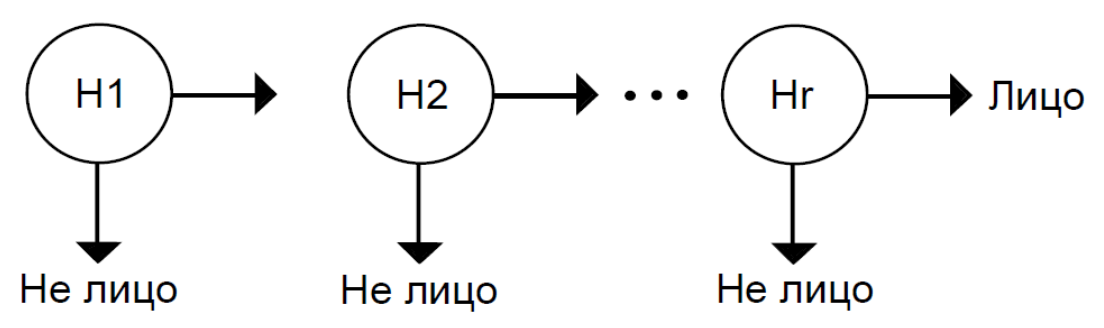
\includegraphics[scale=0.45]{res/pic010}
\caption{Пример вырожденного дерева каскадов}
\end{figure}

Решение каскадного классификатора D может быть записано, как произведение ответов r сильных классификаторов $H_i$:

\begin{gather}
D = \prod\limits_{i=1}^{r} H_i
\end{gather}

Преимущество такого подхода перед одним сильным классификатором объясняется скоростью принятия решений. В качестве эксперимента сильный классификатор, обученный по методу AdaBoost и содержащий 200 признаков, сравнивался с каскадным классификатором, состоящим из 10 уровней по 20 признаков на каждом. В то время как TPR отличался на 2-3\% в пользу сильного классификатора, производительность каскада была почти в 10 раз выше.

\subsection{Смеси гауссовых распределений}

Рассмотрим матрицу X, по столбцам которой расположены вектора признаков изображения. Предполагается, что распределение каждого элемента вектора признаков подчиняется нормальному, поскольку при построении тот подвержен влиянию огромного числа случайных факторов. В качестве генеративного метода, моделирующего характеристики наблюдаемого объекта и среды наблюдения, хорошо зарекомендовали себя смеси гауссовых распределений (СГР). Модель гауссовых смесей может быть записана следующим образом:

\begin{gather}
P(X|\theta) = \sum\limits_{i=1}^{K} a_i \text{Norm}_x[\mu_i,\Sigma_i]
\end{gather}

\begin{gather}
\text{Norm}_x[\mu_i,\Sigma_i]=\frac{1}{(2\pi)^\frac{D}{2} |\Sigma_i|^\frac{1}{2}}e^{-\frac{1}{2}(X-\overline{\mu}_i)^T \Sigma_i^{-1}(X-\overline{\mu}_i)}
\end{gather}

где $X$ -- $D$-мерный вектор случайных величин, $\overline{\mu}_i$ -- вектор математического ожидания, $\Sigma_i$ -- ковариационная матрица, $\alpha_i$ -- веса смеси: $\sum_{i=1}^{N} \alpha_i = 1$, $\theta = [\alpha_i, \overline{\mu}_i, \Sigma_i]$ -- параметры гауссовой смеси, $K$ -- количество гауссоид.

Для построения СГР используется классический EM-алгоритм (Expectation-maximization algorithm), максимизирующий правдоподобие модели на заданных обучающих данных. На E-шаге вычисляется ожидаемое значение функции правдоподобия, при этом скрытые переменные рассматриваются как наблюдаемые (43). На M-шаге рассчитывается оценка максимального правдоподобия, таким образом, увеличивается ожидаемое правдоподобие, вычисляемое на E-шаге. Производится переоценка вектора параметров, используя текущее значение вектора скрытых переменных (44)-(46).

\begin{gather}
\gamma_{nk} = \frac{\alpha_k \text{Norm}_{X_n}[\mu_k,\Sigma_k]}{\sum_{j=1}^{K} \alpha_j \text{Norm}_{X_n}[\mu_k,\Sigma_k]}
\end{gather}

\begin{gather}
\hat{\mu}_k = \frac{1}{N_k} \sum\limits_{n=1}^{N} \gamma_{nk} X_n
\end{gather}

\begin{gather}
\hat{\Sigma}_k = \frac{1}{N_k} \sum\limits_{n=1}^{N} \gamma_{nk} (X_n - \hat{\mu}_k) (X_n - \hat{\mu}_k)^T
\end{gather}

\begin{gather}
\hat{\alpha}_k = \frac{N}{N_k}
\end{gather}

где $N_k = \sum_{n=1}^{N} \gamma_{nk}$, N -- количество элементов обучающей выборки. Пример итеративной сходимости алгоритма показан на рисунке 11.

При обучении модели гауссовых смесей необходимо провести инициализацию параметров модели перед первой итерацией. Не гарантируется нахождение глобального максимума в пространстве данных обучения, таким образом, результат обучения системы в значительной степени зависит от начальных значений. Предположим, что число гауссоид $K$ заранее задано, тогда для инициализации параметров $[\alpha_i, \overline{\mu}_i, \Sigma_i]$ может использоваться случайная инициализация параметров модели, алгоритм $k$-средних, метод главных компонент и др.

\begin{figure}[h!]
\centering
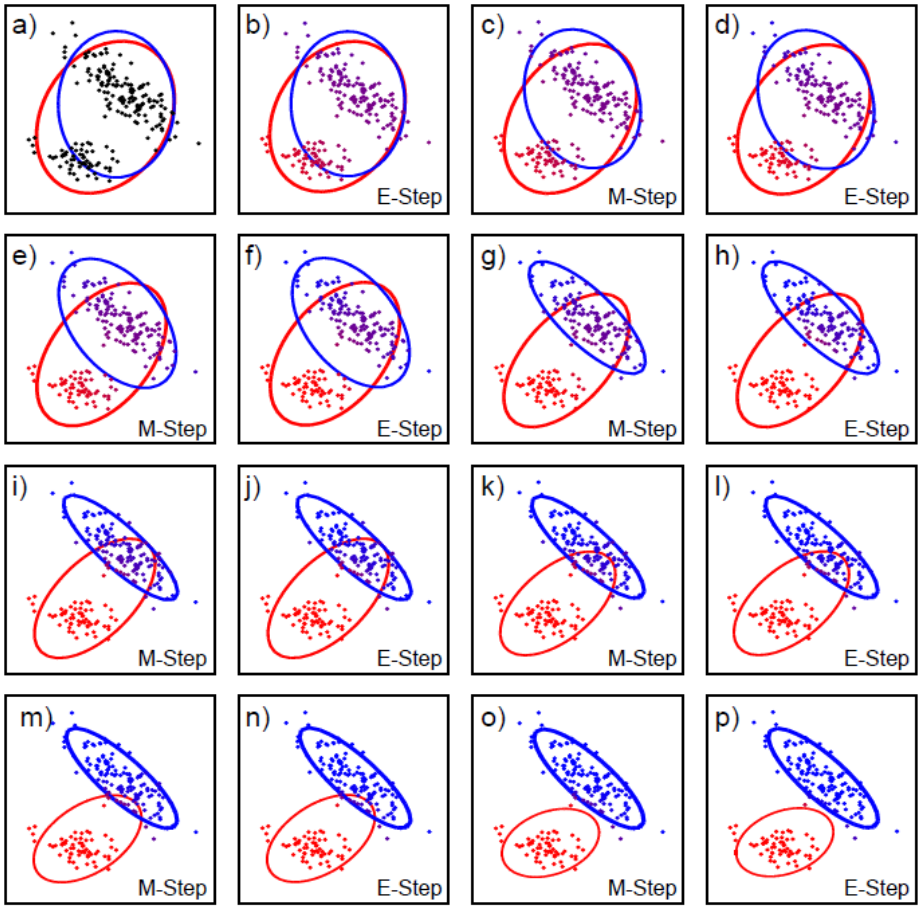
\includegraphics[scale=0.4]{res/pic011}
\caption{a) Исходная модель. b) E-шаг. Для каждой точки плоскости была рассчитана постериорная вероятность, порожденная из каждой гауссоиды (обозначена соответствующим цветом). с) M-шаг. Обновлены среднее, дисперсия и веса каждой гауссоиды согласно постериорным вероятностям Эллипсы отображают расстояние Махаланобиса, их толщина -- вес гауссоиды. d)-t) Череда E- и M-шагов.}
\end{figure}

При обучении СГР-модели важно предупредить случаи, когда эллипсы гауссоид могут превратиться в точку (проблема "схлопывания гауссоид") или покрыть всю выборку. Для предотвращения этого обычно вводят ограничения на элементы дисперсионной матрицы $\Sigma_i$.

%------------------------------------------------------------------------------

\newpage
\section{Нейронные сети}

Среди алгоритмов распознавания образов особое место занимают нейронные сети. Повышенный интерес к данной технологии в наши дни обусловлен успехами сетей в распознавании широкого класса паттернов, новыми численными методами для обучения многоуровневых нелинейных моделей и прогрессом в области производства недорогих и эффективных векторных процессоров для расчетов. При решении задач компьютерного зрения наибольшей популярностью пользуются сверточные нейронные сети (СНС). Модель СНС улучшает качество распознавания каскадного классификатора на ЛБШ за счет дополнительной фильтрации шумов.

В середине прошлого столетия ученые Торстен Визель и Дэвид Хьюбел исследовали зрительную кору головного мозга кошки и обнаружили, что существует два различных типа клеток. Так называемые простые клетки реагируют на прямые линии (полосы света, края стимулов) под определенным углом. Сложные клетки реагирую на движение линий (полос света, краев стимулов) в определенных направлениях. Спустя некоторое время, это открытие нашло применение в прикладной области информатики: Кунихика Фукусима воплотил идею простых и сложных клеток в неокогнитроне

\begin{figure}[h!]
\centering
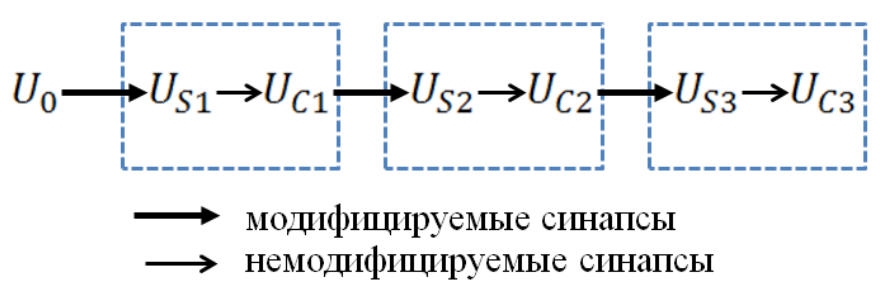
\includegraphics[scale=0.5]{res/pic012}
\caption{Упрощенная структура неокогнитрона}
\end{figure}

Неокогнитрон состоит из ретины (сетчатки) $U_0$ и последовательности групп нейронов, каждая из которых, в свою очередь, содержит два типа нейронных слоев (рис. 12). Простые нейроны (из слоев $U_S$) принимают сигналы от сложных нейронов предыдущего слоя и обнаруживают одинаковые признаки, но в разных местах сигнала. Сложные нейроны (из слоев $U_C$) объединяют отклики простых нейронов из своей группы и стремятся редуцировать зависимость реакции на признаки от их положения. Таким образом, неокогнитрон приобретает способность детектировать определенные комбинации признаков, независимо от их положения на ретине.

\begin{figure}[h!]
\centering
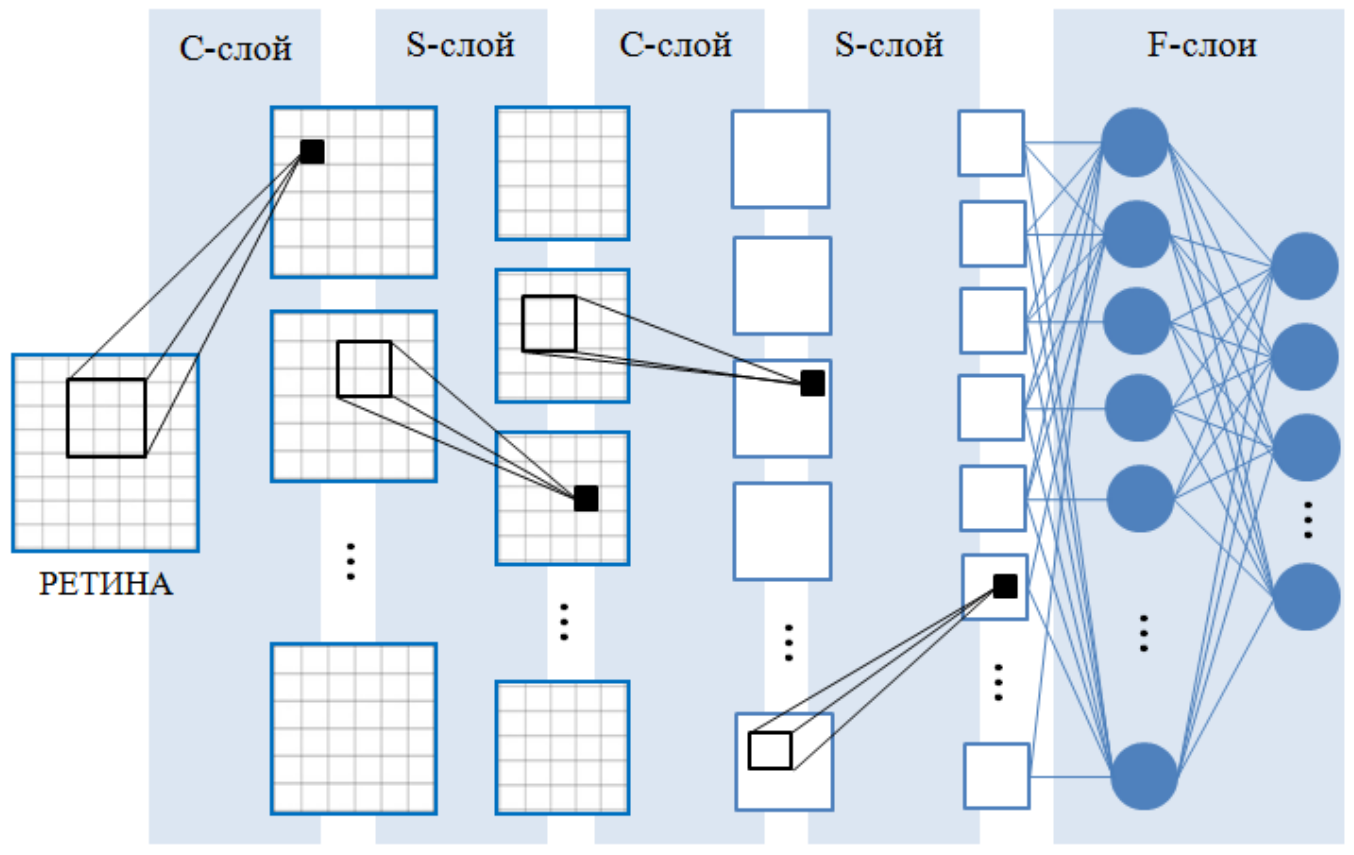
\includegraphics[scale=0.35]{res/pic013}
\caption{Архитектура сверточной нейронной сети}
\end{figure}

Отличие неокогнитрона от многослойного персептрона заключается в трех инновационных для нейронных сетей на тот момент архитектурных принципах:
\begin{itemize}
\item локальные рецептивные поля,
\item разделяемые веса,
\item пространственная субдискретизация.
\end{itemize}

Развивая идею неокогнитрона, Ян ЛеКун вместе с соавторами предложили структуру классической сверточной нейронной сети (СНС) и алгоритм для ее обучения с учителем, а также применение СНС для решения широкого круга задач распознавания образов. СНС, предложенные ЛеКуном (рис. 13), это иерархичные архитектурные многослойные идеи нейронные неокогнитрона, сети, в которых обеспечивающие сходятся некоторую три степень инвариантности представления данных.

Устройство СНС заключается в чередовании сверточных слоев (convolutional, C-слои), реализующих концепцию простых клеток зрительной коры с гибкими (обучаемыми) весами, и субдискретизирующих слоев (sub-sampling, S-слои), построенных по примеру сложных клеток кортекса с жесткими весами. Завершается подобная каскадная модель, как правило, полносвязными нейронными слоями (fully-connected, F-слои). Различные архитектуры СНС успешно используются во многих сложных приложениях, связанных с обработкой визуальных данных.

%------------------------------------------------------------------------------

\newpage
\section{Экспериментальные исследования}

Библиотека Dlib реализует алгоритмы машинного обучения и позволяет использовать описанные выше методы. Библиотека распространяется под свободной лицензией  Boost Software License и включает в себя много полезных классов и функций. Основные возможности:
\begin{itemize}
\item Потоки (переносимый API для работы с потоками, межпотоковое взаимодействие по средствам pipe, локальные данные потока, пул потоков, механизм запуска глобальных функций в отдельном потоке и др.)
\item Сетевое программирование (переносимый API для работы с TCP сокетами, TCP сервер, HTTP сервер и др.)
\item Графический интерфейс пользователя (переносимый и потокобезопасный GUI API)
\item Численные алгоритмы (матрицы и операции над ними, алгоритмы нелинейной оптимизации, целые числа с диапазоном ограниченным только ресурсами системы, генератор псевдослучайных чисел и др.)
\item Алгоритмы машинного обучения
\item Алгоритмы для вычислений и обучения байесовских сетей.
\item Обработка изображений (чтение и запись формата Windows BMP, выделение границ, компьютерное зрение и др.).
\item Алгоритмы сжатия и проверки целостности (CRC32, MD5, LZP и др.).
\item Тестирование (потокобезопасный класс ведения лога, модельное тестирование, макросы проверки предусловий).
\item Полезные классы общего назначения (разбор XML, разбор параметров командной строки, различные контейнеры, base64 и др.). 
\end{itemize}

Для простоты, воспользуемся языком программирования Python (листинг 1). Этот скрипт умеет определять множество лиц на одном изображении.

\lstinputlisting[language=Python, caption={Пример простого скрипта для определения лица}]{res/detector.py}

\begin{figure}[h!]
\centering
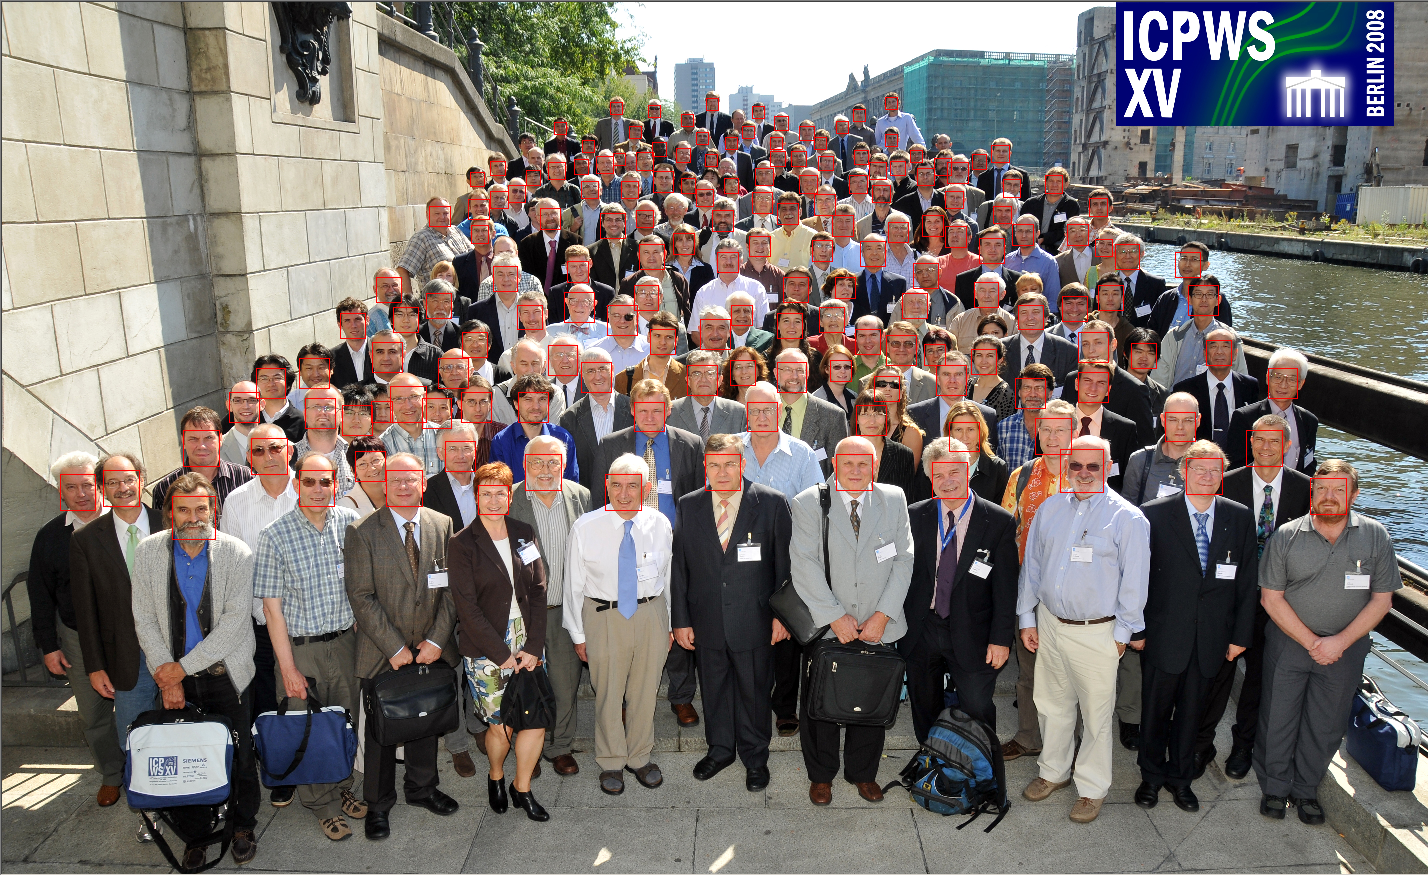
\includegraphics[scale=0.35]{res/pic014}
\caption{Определение множества лиц}
\end{figure}

\begin{figure}[h!]
\centering
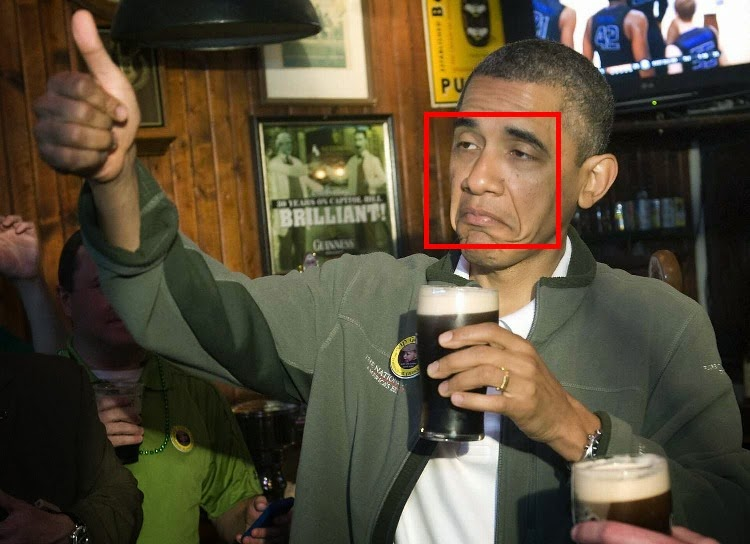
\includegraphics[scale=0.6]{res/pic015}
\caption{Определение одного лица}
\end{figure}

На рисунках 14 и 15 представлены результаты работы скрипта. Предложенный метод детектирования позволяет уверенно обнаруживать большую часть лиц на фотографиях, включая лица с большим углом отклонения.

Для встраиваемых решений подобный подход может оказаться избыточным, но для классической обработки изображений на сервере с архитектурой x86\_64 реализована оптимальная поддержка со стороны аппаратуры, результатом чего является высокое быстродействие и хороший показатель определения лиц.


%------------------------------------------------------------------------------

\newpage
\section*{Заключение}
\addcontentsline{toc}{section}{Заключение}

В данной работе рассмотрены наиболее распространенные методы выделения информативных признаков цифровых изображений, такие как признаки Хаара, ЛБШ, дискретное косинусное преобразование. Представлены базовые алгоритмы классификации признаков в постановке задачи детектирования. Приведён краткий обзор работы нейронной сети.

В практической части представлен скрипт на языке Python с использованием библиотеки dlib и результаты определения лиц на нескольких изображениях.

%------------------------------------------------------------------------------

\newpage
\section*{Список литературы}
\addcontentsline{toc}{section}{Список литературы}

\begin{enumerate}
\item Вежневец В. Обнаружение и локализация лица на изображении.
\item Тимошенко Д.М. Методы автоматической идентификации личности по изображениям лиц, полученным в неконтролируемых условиях.
\item Vladimir Vezhnevets. Method For Localization Of Human Faces In Color-Based Face Detectors And Trackers.
\item Sung H. Yoon, Gi T. Hur, and Jung H. Kim. Recurrent Neural Network Verifier for Face Detection and Tracking
\item Karin Sobottka, Ioannis Pitas. Segmentation and Tracking of Faces in Color Images.
\item Fu Jie Huang, Tsuhan Chen. Tracking of Multiple Faces for Human-Computer Interfaces and Virtual Environments.
\item Бустинг // MachineLearning.ru: [сайт]. URL: http://goo.gl/rvF45r
\end{enumerate}


\end{document}
